\documentclass[main-ap-physics.tex]{subfiles}
\usetikzlibrary{decorations.markings}

\begin{document}

\subsubsection*{Adding Vectors Using Analytical Methods}

To see how to add vectors using perpendicular components, consider Figure \ref{i2ER22}, in which the vectors \textbf{A} and \textbf{B} are added to produce the resultant \textbf{R}.


\begin{center}
    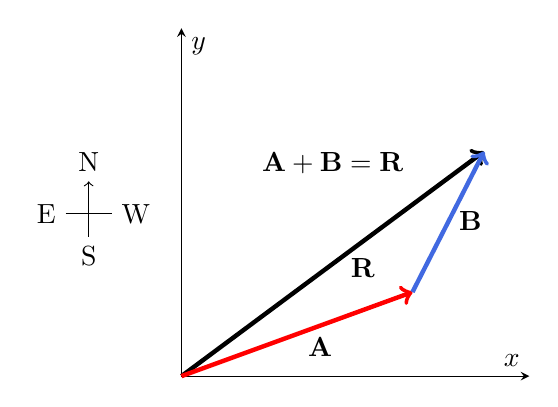
\begin{tikzpicture}
        \begin{axis}[width=6cm,height=6cm,
            axis lines=center,
            xmin=0,xmax=75,
            ymin=0,ymax=75,
            ticks=none,
            clip=false,
            xlabel=$x$,
            ylabel=$y$
        ]
        \coordinate (R) at ({81.2*cos(36.6)},{81.2*sin(36.6)});
        \coordinate (A) at ({53*cos(20)},{53*sin(20)});
        \coordinate (B) at ({34*cos(63)},{34*sin(63)});
        \draw[ultra thick,->] (0,0) -- (R) node[below=2pt,pos=0.6] {\textbf{R}} node[above=1cm,pos=0.5] {$\textbf{A} + \textbf{B} = \textbf{R}$};
        \draw[ultra thick,->,red] (0,0) -- (A) node[below,pos=0.6,black] {\textbf{A}};
        \draw[ultra thick,->,RoyalBlue] (A) -- ++(B) node[below right=-1mm,pos=0.6,black] {\textbf{B}};
        \begin{scope}[shift={(-20,30)}]
            \draw[->] (0,0) node[below] {S} -- ++(0,12) node[above] {N};
            \draw (-5,5) node[left] {E} -- ++(10,0) node [right] {W};
        \end{scope}
        \end{axis}
    \end{tikzpicture}
    \captionsetup{type=figure,margin=1in,font=scriptsize}
    \captionof{figure}{Vectors \textbf{A} and \textbf{B} are two legs of a walk, and \textbf{R} is the resultant or total displacement. You can use analytical methods to determine the magnitude and direction of \textbf{R}.}
    \label{i2ER22}
\end{center}

If \textbf{A} and \textbf{B} represent two legs of a walk (two displacements), then \textbf{R} is the total displacement. The person taking the walk ends up at the tip of \textbf{R}. There are many ways to arrive at the same point. In particular, the person could have walked first in the $x$-direction and then in the $y$-direction. Those paths are the $x$- and $y$-components of the resultant, $\textbf{R}_x$ and $\textbf{R}_y$. If we know $\textbf{R}_x$ and $\textbf{R}_y$, we can find $R$ and $\theta$ using the equations $A = \sqrt{A_x^2 + A_y^2}$ and $\theta = \tan^{-1} (A_y/A_x)$. When you use the analytical method of vector addition, you can determine the components or the magnitude and direction of a vector.

\vspace{1em}

\textbf{Step 1}. \textit{Identify the x- and y-axes that will be used in the problem. Then, find the components of each vector to be added along the chosen perpendicular axes}. Use the equations $A_x = A \cos{\theta}$ and $A_y = A \sin{\theta}$ to find the components. In Figure \ref{0kxQWq}, these components are $A_x$, $A_y$, $B_x$, and $B_y$. The angles that vectors \textbf{A} and \textbf{B} make with the $x$-axis are $\theta_{\text{A}}$ and $\theta_{\text{B}}$, respectively.

\begin{center}
    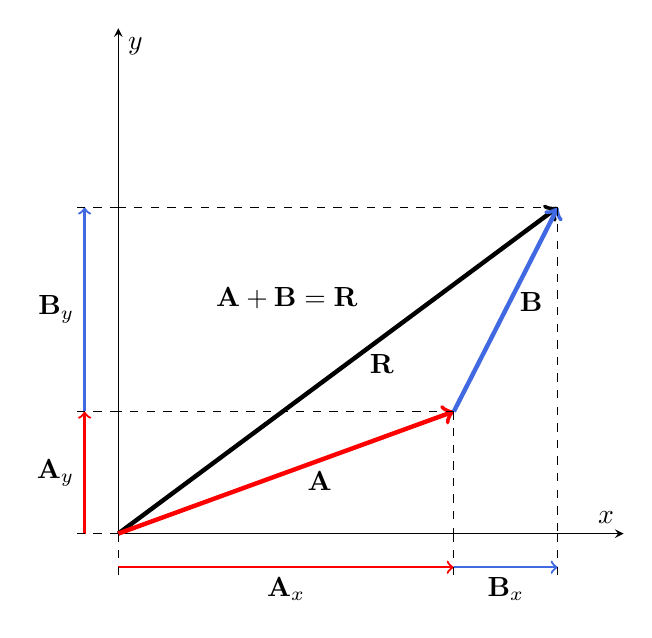
\begin{tikzpicture}
        \begin{axis}[width=8cm,height=8cm,
            axis lines=center,
            xmin=0,xmax=75,
            ymin=0,ymax=75,
            ticks=none,
            clip=false,
            xlabel=$x$,
            ylabel=$y$
        ]
        \coordinate (R) at ({81.2*cos(36.6)},{81.2*sin(36.6)});
        \coordinate (Rx) at ({81.2*cos(36.6)},0);
        \coordinate (A) at ({53*cos(20)},{53*sin(20)});
        \coordinate (Ax) at ({53*cos(20)},0);
        \coordinate (Ay) at (0,{53*sin(20)});
        \coordinate (B) at ({34*cos(63)},{34*sin(63)});
        \coordinate (Bx) at ({34*cos(63)},0);
        \coordinate (By) at (0,{34*sin(63)});
        \draw[ultra thick,->] (0,0) -- (R) node[below=2pt,pos=0.6] {\textbf{R}};
        \node at (25,35) {$\textbf{A} + \textbf{B} = \textbf{R}$};
        \draw[ultra thick,->,red] (0,0) -- (A) node[below,pos=0.6,black] {\textbf{A}};
        \draw[ultra thick,->,RoyalBlue] (A) -- ++(B) node[below right=-1mm,pos=0.6,black] {\textbf{B}};
        
        \draw[dashed] (R) -- ++({-81.2*cos(36.6)},0);
        \draw[dashed] (A) -- ++({-53*cos(20)},0);
        \draw[thick,red,->] (-5,0) -- ++(Ay) node[left,black,pos=0.5] {$\textbf{A}_y$};
        \draw[thick,RoyalBlue,->] (-5,{53*sin(20)}) -- ++(By) node[left,black,pos=0.5] {$\textbf{B}_y$};
        \draw[dashed] (0,{53*sin(20)+34*sin(63)}) -- ++(-7,0);
        \draw[dashed] (0,{53*sin(20)}) -- ++(-7,0);
        \draw[dashed] (0,0) -- ++(-7,0);

        \draw[dashed] (R) -- ++(0,{-81.2*sin(36.6)});
        \draw[dashed] (A) -- ++(0,{-53*sin(20)});
        \draw[thick,red,->] (0,-5) -- ++(Ax) node[below,black,pos=0.5] {$\textbf{A}_x$};
        \draw[thick,RoyalBlue,->] ({53*cos(20)},-5) -- ++(Bx) node[below,black,pos=0.5] {$\textbf{B}_x$};
        \draw[dashed] (0,0) -- ++(0,-7);
        \draw[dashed] ({53*cos(20)+34*cos(63)},0) -- ++(0,-7);
        \draw[dashed] ({53*cos(20)},0) -- ++(0,-7);
        

        % \begin{scope}[shift={(-20,30)}]
        %     \draw[->] (0,0) node[below] {S} -- ++(0,12) node[above] {N};
        %     \draw (-5,5) node[left] {E} -- ++(10,0) node [right] {W};
        % \end{scope}
        \end{axis}
    \end{tikzpicture}
    \captionsetup{type=figure,margin=1in,font=scriptsize}
    \captionof{figure}{To add vectors \textbf{A} and \textbf{B}, first determine the horizontal and vertical components of each vector. These are the dotted vectors $\textbf{A}_x$, $\textbf{A}_y$, $\textbf{B}_x$ and $\textbf{B}_y$ shown in the image.}
    \label{0kxQWq}
\end{center}

\textbf{Step 2}. \textit{Find the components of the resultant along each axis by adding the components of the individual vectors along that axis}. That is, as shown in Figure \ref{QVly9l},

\begin{equation*}
    R_x = A_x + B_x
\end{equation*}

and

\begin{equation*}
    R_y = A_y + B_y
\end{equation*}


\begin{center}
    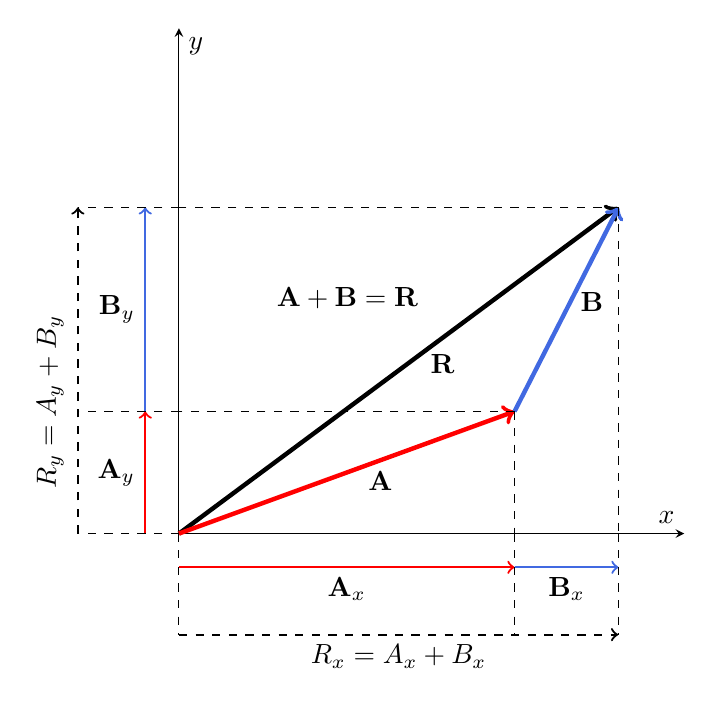
\begin{tikzpicture}
        \begin{axis}[width=8cm,height=8cm,
            axis lines=center,
            xmin=0,xmax=75,
            ymin=0,ymax=75,
            ticks=none,
            clip=false,
            xlabel=$x$,
            ylabel=$y$
        ]
        \coordinate (R) at ({81.2*cos(36.6)},{81.2*sin(36.6)});
        \coordinate (Rx) at ({81.2*cos(36.6)},0);
        \coordinate (Ry) at (0,{81.2*sin(36.6)});
        \coordinate (A) at ({53*cos(20)},{53*sin(20)});
        \coordinate (Ax) at ({53*cos(20)},0);
        \coordinate (Ay) at (0,{53*sin(20)});
        \coordinate (B) at ({34*cos(63)},{34*sin(63)});
        \coordinate (Bx) at ({34*cos(63)},0);
        \coordinate (By) at (0,{34*sin(63)});
        \draw[ultra thick,->] (0,0) -- (R) node[below=2pt,pos=0.6] {\textbf{R}};
        \node at (25,35) {$\textbf{A} + \textbf{B} = \textbf{R}$};
        \draw[ultra thick,->,red] (0,0) -- (A) node[below,pos=0.6,black] {\textbf{A}};
        \draw[ultra thick,->,RoyalBlue] (A) -- ++(B) node[below right=-1mm,pos=0.6,black] {\textbf{B}};
        
        \draw[dashed] (R) -- ++({-81.2*cos(36.6)},0);
        \draw[dashed] (A) -- ++({-53*cos(20)},0);
        \draw[thick,red,->] (-5,0) -- ++(Ay) node[left,black,pos=0.5] {$\textbf{A}_y$};
        \draw[thick,RoyalBlue,->] (-5,{53*sin(20)}) -- ++(By) node[left,black,pos=0.5] {$\textbf{B}_y$};
        \draw[dashed] (0,{53*sin(20)+34*sin(63)}) -- ++(-15,0);
        \draw[dashed] (0,{53*sin(20)}) -- ++(-15,0);
        \draw[dashed] (0,0) -- ++(-15,0);
        
        \draw[thick,dashed,->] (-15,0) -- ++(Ry) node[left=3.5mm,pos=0.7,rotate=90] {$R_y = A_y + B_y$};

        \draw[dashed] (R) -- ++(0,{-81.2*sin(36.6)});
        \draw[dashed] (A) -- ++(0,{-53*sin(20)});
        \draw[thick,red,->] (0,-5) -- ++(Ax) node[below,black,pos=0.5] {$\textbf{A}_x$};
        \draw[thick,RoyalBlue,->] ({53*cos(20)},-5) -- ++(Bx) node[below,black,pos=0.5] {$\textbf{B}_x$};
        \draw[dashed] (0,0) -- ++(0,-15);
        \draw[dashed] ({53*cos(20)+34*cos(63)},0) -- ++(0,-15);
        \draw[dashed] ({53*cos(20)},0) -- ++(0,-15);

        \draw[thick,dashed,->] (0,-15) -- ++(Rx) node[below,pos=0.5] {$R_x = A_x + B_x$};
        \end{axis}
    \end{tikzpicture}
    \captionsetup{type=figure,margin=1in,font=scriptsize}
    \captionof{figure}{The magnitude of the vectors $\textbf{A}_x$ and $\textbf{B}_x$ add to give the magnitude $R_x$ of the resultant vector in the horizontal direction. Similarly, the magnitudes of the vectors $\textbf{A}_y$ and $\textbf{B}_y$ add to give the magnitude $R_y$ of the resultant vector in the vertical direction.}
    \label{QVly9l}
\end{center}

Components along the same axis, say the $x$-axis, are vectors along the same line and, thus, can be added to one another like ordinary numbers. The same is true for components along the $y$-axis. (For example, a 9-block eastward walk could be taken in two legs, the first 3 blocks east and the second 6 blocks east, for a total of 9, because they are along the same direction.) So resolving vectors into components along common axes makes it easier to add them. Now that the components of \textbf{R} are known, its magnitude and direction can be found.

\vspace{1em}

\textbf{Step 3}. \textit{To get the magnitude \textbf{R} of the resultant, use the Pythagorean theorem:}

\begin{equation}
    R = \sqrt{R_x^2 + R_y^2}
\end{equation}

\textbf{Step 4}. \textit{To get the direction of the resultant relative to the $x$-axis:}

\begin{equation}
    \theta = \tan^{-1}\left(\frac{R_y}{R_x}\right)
\end{equation}

The following example illustrates this technique for adding vectors using perpendicular components.



\end{document}



